\documentclass{article}
\usepackage[italian]{babel}
\usepackage[utf8x]{inputenc}
\usepackage[T1]{fontenc}
\usepackage{graphicx}
\usepackage[colorlinks=true, allcolors=unimorered]{hyperref} %sets hyperlink colour
\usepackage{caption}
\usepackage{subcaption}
\usepackage{xcolor}
\usepackage{roboto} % for Roboto Slab font
\usepackage{float}
\usepackage{titling}
\usepackage{titlesec}
\usepackage[square,sort,comma,numbers]{natbib}
\usepackage{tikz}
\usepackage{geometry}
\usepackage{sectsty}
\usepackage{amsmath}
\usepackage{tikzpagenodes}
\usepackage{booktabs}
\usepackage{listings}
\usepackage{siunitx}
\sisetup{group-separator={.},group-minimum-digits=4}
\geometry{a4paper, margin=2cm}
\definecolor{unimorered}{RGB}{209,65,36}
\definecolor{unimoregrey}{RGB}{99,102,106}
\definecolor{codebg}{RGB}{245,245,245}
\allsectionsfont{\color{black}} %sets colour for all headers
\usepackage{helvet}
\renewcommand{\familydefault}{\sfdefault}
\sectionfont{\fontfamily{RobotoSlab-TLF}\selectfont}

% --- listings style for Mongo/JS pipelines ---
\lstdefinestyle{mongo}{
    backgroundcolor=\color{codebg},
    basicstyle=\ttfamily\footnotesize,
    keywordstyle=\color{unimorered},
    commentstyle=\color{unimoregrey}\itshape,
    breaklines=true,
    frame=single,
    rulecolor=\color{unimoregrey},
    framesep=5pt,
    xleftmargin=5pt,
    showstringspaces=false,
    columns=fullflexible
}
\lstset{style=mongo}
%%%%%%%%%%%%%%%%%%%%%%%%%%%%%%%%%%%%%%%%%%%%%%%%%%%%%%%%%
\begin{document}

\input{titlepage}

%%% Create a table of contents
\tableofcontents
\newpage

%==================================================================
\addcontentsline{toc}{section}{Abstract}
\section*{Abstract}
Questa relazione presenta un approfondimento sperimentale su \textbf{MongoDB}, il
sistema NoSQL documentale più diffuso, condotto su un dataset reale di programmi
di allenamento (Boostcamp, Kaggle): \num{605033} righe in formato piatto e
denormalizzato, con una struttura logica gerarchica a quattro livelli
\emph{programma $\rightarrow$ settimana $\rightarrow$ giorno $\rightarrow$ esercizio}.
L'intera analisi gira contro un \textbf{replica set a 3 nodi} avviato con Docker
Compose, che nella parte finale diventa anche il banco di prova per il teorema CAP.
La sperimentazione è organizzata attorno a quattro \emph{research question}:
(RQ1) la convenienza di rimodellare il dataset piatto in documenti annidati
(\emph{embedding vs referencing}); (RQ2) l'uso dell'aggregation framework per fare
analytics direttamente nel database; (RQ3) l'impatto degli indici sulle
performance, misurato con \texttt{explain("executionStats")}; (RQ4) il
comportamento del sistema sotto partizione di rete, osservato uccidendo dal vivo
il nodo primario. I risultati principali: l'embedding riduce i dati logici del
\textbf{87\%} (da 414 a 54~MB) e abbatte la latenza di lettura di due ordini di
grandezza; gli indici fanno crollare i documenti esaminati da \num{605033} a zero
nel caso di \emph{covered query}; il failover dal vivo mostra che MongoDB è un
sistema \textbf{CP}, che sotto partizione sacrifica la disponibilità in scrittura
per preservare la consistenza. Tutto il codice e le istruzioni di riproduzione
sono pubblicati su un repository GitHub corredato di README.

%==================================================================
\section{Introduzione e contesto}
\label{sec:intro}

Per l'approfondimento sui sistemi NoSQL ho scelto \textbf{MongoDB}, un database
citato a lezione che si basa su dati semi strutturati. Il modello utilizzato da
MongoDB rinuncia allo schema rigido, tipico degli RDBMS, in favore di documenti
BSON annidati~\cite{MongoDBDefinitiveGuide}. In questo approfondimento andremo a
capire quando questo modello conviene davvero, quali garanzie offre e a cosa
rinuncia, dato che sappiamo dal teorema CAP che non si possono garantire tutti e
tre i principi.

\paragraph{Il dataset.} Come caso di studio uso un dataset Kaggle di programmi di
allenamento della piattaforma Boostcamp~\cite{BoostcampDataset}, composto da
\num{605033} righe, una per esercizio. Il CSV è completamente
\textbf{denormalizzato}, quindi ogni riga ripete tutti i metadati del programma
(titolo, descrizione, livello, obiettivo, equipment, \dots). I dati però hanno una
gerarchia naturale a quattro livelli,
\emph{programma $\rightarrow$ settimana $\rightarrow$ giorno $\rightarrow$ esercizio},
ed è proprio questo che mi ha spinto a voler utilizzare un'architettura NoSQL
documentale. Per la simulazione d'analisi ho virtualizzato 3 nodi MongoDB su
container Docker.

\paragraph{Le research question.} Le domande che mi sono posto sono quattro,
ciascuna sperimentata e misurata sul replica set:
\begin{itemize}
    \item \textbf{RQ1 --- Modellazione:} conviene rimodellare il dataset piatto in
    documenti annidati o possiamo lasciarli standard? Confronto spazio e accesso.
    \item \textbf{RQ2 --- Aggregation framework:} che analisi si possono fare
    \emph{direttamente nel database} con le pipeline di aggregazione, senza
    estrarre i dati?
    \item \textbf{RQ3 --- Indici:} che impatto possono avere gli indici supportati
    da MongoDB? Anche in questo assignment profilo le query.
    \item \textbf{RQ4 --- Teorema CAP:} come si comporta il replica set sotto
    partizione? Vediamo scenari in cui i nodi falliscono.
\end{itemize}

La Sezione~\ref{sec:metodo} descrive l'infrastruttura sperimentale; le
Sezioni~\ref{sec:rq1}--\ref{sec:rq4} rispondono alle quattro RQ con i risultati
ottenuti; la Sezione~\ref{sec:conclusioni} riassume cosa è stato provato e la sua
rilevanza.

%==================================================================
\section{Metodologia e setup sperimentale}
\label{sec:metodo}

L'intera sperimentazione è riproducibile da un notebook Jupyter
(\texttt{fitness\_exercise\_analysis.ipynb}) che si connette, come sorgente unica,
a un \textbf{replica set \texttt{rs0} a 3 nodi} avviato con Docker
Compose~\cite{MongoDBReplication}. I tre processi \texttt{mongod} ascoltano sulle
porte 27017/27018/27019 e condividono la rete, così da essere raggiungibili come
\texttt{localhost:2701x} sia tra container sia dall'host. La connection string in
\texttt{.env} elenca tutti e tre i membri:

\begin{lstlisting}[language=, caption={Connection string del replica set.}]
mongodb://localhost:27017,localhost:27018,localhost:27019/?replicaSet=rs0
\end{lstlisting}

Il driver PyMongo scopre da solo la topologia e indirizza le operazioni al nodo
giusto. Interrogando \texttt{replSetGetStatus} vediamo che sono stati correttamente
creati 3 container Docker (ovviamente in locale) in ascolto su porte diverse.
Notiamo anche che uno è stato eletto \textbf{PRIMARY}, e sarà il nodo che riceverà
tutte le scritture, mentre gli altri due sono di default diventati
\textbf{SECONDARY}, che replicheranno in modo asincrono a meno che le richieste
non siano specifiche su nodi secondary (cosa che sfrutterò nella RQ4).

\paragraph{Ingestione.} Importo il CSV piatto nella collection \texttt{workouts},
una riga per esercizio, a batch di \num{5000} documenti via
\texttt{insert\_many}. Due accortezze in fase di import: (i) le colonne
\texttt{level} e \texttt{goal} contengono liste serializzate come stringhe (es.
\texttt{"['Beginner', 'Novice']"}), le riconverto in veri array, che BSON
memorizza come array nativi, fondamentale per poterci fare \texttt{\$unwind} nella
RQ2; (ii) le date diventano \texttt{datetime} e i pochi valori mancanti diventano
\texttt{None}, cioè BSON \texttt{null}. Su un replica set il write concern di
default è \texttt{w:"majority"}: ogni batch è confermato solo quando la
maggioranza dei nodi (2 su 3) ha applicato la scrittura, quindi la durabilità è
garantita anche se un nodo cade subito dopo l'import. La collection
\texttt{workouts} riproduce fedelmente il CSV: il punto di partenza
\emph{denormalizzato}, volutamente inefficiente, su cui costruire RQ1.

L'ambiente software è Python~3.11+ con \texttt{pymongo}, \texttt{pandas},
\texttt{python-dotenv}, \texttt{matplotlib} e \texttt{seaborn}; le misure di
tempo e di storage sono ottenute con gli strumenti diagnostici nativi di MongoDB
(\texttt{collStats}, \texttt{explain}, \texttt{replSetGetStatus}). I valori
numerici riportati sono quelli osservati su una singola macchina con i tre nodi in
locale: contano gli ordini di grandezza e i rapporti relativi, non i millisecondi
assoluti.

%==================================================================
\section{RQ1 --- Modellazione: dal CSV piatto ai documenti annidati}
\label{sec:rq1}

Nel CSV ogni esercizio ripete \emph{tutti} i metadati del suo programma: per un
programma con 230 esercizi, titolo, descrizione, livello e obiettivo sono
duplicati 230 volte. In un database relazionale normalizzerei in quattro tabelle
(programs, weeks, days, exercises) e ricostruirei il programma con tre join.
MongoDB offre una terza via, l'\textbf{embedding}: un documento per programma, con
la gerarchia settimane~$\rightarrow$~giorni~$\rightarrow$~esercizi annidata dentro.

Avrei potuto scegliere, invece dell'embedding, il \textbf{referencing} (documenti
separati con riferimenti, lo stile ``relazionale'' di MongoDB), ma dato che quando
si parla di piani di allenamento il pattern di accesso è per \emph{l'intero piano}
e non per i sotto-oggetti, ha più senso proseguire con l'embedding. Dunque
costruisco la collection \texttt{programs}, senza far uscire i dati dal database,
con una pipeline che aggrega giorno $\rightarrow$ settimana $\rightarrow$ programma
e termina in \texttt{\$out}:

\begin{lstlisting}[language=, caption={Schema della pipeline di rimodellazione (semplificato).}]
[ {$group: {_id:{prog,week,day}, exercises:{$push:...}}},   // giorno
  {$group: {_id:{prog,week}, days:{$push:...}}},            // settimana
  {$group: {_id:"$prog", weeks:{$push:...}}},               // programma
  {$addFields: {weeks: {$sortArray: ...}}},  // ordino settimane e giorni
  {$out: "programs"} ]   // allowDiskUse=True
\end{lstlisting}

Notiamo come dai \num{605033} documenti di partenza sia riuscito a collassarli in
\textbf{\num{2598} documenti} unici, dato che il titolo fa da chiave naturale
(\texttt{\_id}) e quindi l'unicità è garantita dal database. Ho impostato
\texttt{allowDiskUse=True} in quanto, data la mole di documenti, i \texttt{\$group}
superano il limite di default di MongoDB di 100~MB di RAM per stage: in questo modo
permettiamo lo spilling su disco. Inoltre, dato che \texttt{\$push} non garantisce
l'ordine degli elementi, ho aggiunto uno stage finale con \texttt{\$sortArray} che
riordina settimane e giorni prima del \texttt{\$out}.

Ogni singolo documento della collezione risultante è costituito come segue:
\begin{itemize}
    \item Programma (id univoco che fa da chiave);
    \item Equipaggiamento;
    \item Livello di esperienza;
    \item Durata in settimane;
    \item Giorni per settimana;
    \item Esercizi per giorno (ognuno con i suoi campi: name, sets, reps,
    intensity).
\end{itemize}
Per esempio il programma \emph{Weightlifting Mobility program} diventa un singolo
documento con equipment, livelli, 7 settimane, ognuna con i suoi giorni e dentro
ogni giorno i suoi esercizi. Nessuna ricostruzione applicativa, nessun join.

\begin{table}[H]
\centering
\caption{Confronto tra rappresentazione piatta (\texttt{workouts}) e annidata
(\texttt{programs}).}
\label{tab:storage}
\begin{tabular}{lrrr}
\toprule
Metrica & Piatta (\texttt{workouts}) & Annidata (\texttt{programs}) & Variazione \\
\midrule
Documenti              & \num{605033} & \num{2598} & $-99.6\%$ \\
Dati logici            & 413{,}8 MB   & 54{,}4 MB  & $\mathbf{-87\%}$ \\
Storage su disco       & 45{,}3 MB    & 7{,}4 MB   & $-84\%$ \\
Dim. media documento   & 0{,}7 KB     & $\sim$21 KB & --- \\
Lettura ``programma X''& $\sim$165 ms (325 doc) & $\sim$1{,}2 ms (1 doc) & $\mathbf{\sim 100\times}$ \\
\bottomrule
\end{tabular}
\end{table}

Il confronto (Tabella~\ref{tab:storage}) quantifica i due vantaggi dell'embedding
su questo dataset:
\begin{enumerate}
    \item \textbf{Storage:} ho ridotto notevolmente i dati memorizzati collassando
    i documenti, al costo di aumentare la dimensione del documento singolo, che
    resta comunque molto sotto la soglia dei \textbf{16~MB} massimi previsti per
    singolo documento (il vincolo strutturale da verificare sempre prima di
    scegliere l'embedding).
    \item \textbf{Pattern di accesso:} l'intero programma si recupera con una
    lettura di un singolo documento ($\sim$1{,}2~ms, servita dall'indice di default
    su \texttt{\_id}); nella versione piatta servono 325 documenti da filtrare, e
    senza indice questo comporta una scansione completa dei 605k documenti
    ($\sim$165~ms), da riassemblare poi lato applicazione. L'accesso al documento è
    inoltre \textbf{atomico}: una modifica al programma intero non richiede
    transazioni multi-documento, in quanto i dati sono stati raggruppati.
\end{enumerate}

\paragraph{Quando invece conviene il referencing?} Se i sotto-oggetti fossero
acceduti indipendentemente dal padre (es. ``tutti i giorni di allenamento di oggi,
di qualunque programma'') allora valuterei uno schema referencing. È il classico
trade-off del modello documentale: \emph{si modella in base a come si legge}, non
in base alla struttura ``pura'' dei dati.

\paragraph{Risposta a RQ1.} Sì: per questo dataset, con questo pattern di accesso,
il modello annidato è superiore su storage, semplicità e atomicità.

%==================================================================
\section{RQ2 --- Aggregation framework: analytics nel database}
\label{sec:rq2}

Inizio dalla domanda più naturale: \emph{quali sono gli esercizi più usati nei
programmi?} Dal momento in cui ho compattato i documenti, per rispondere è
necessario utilizzare la soluzione proposta da MongoDB, l'\textbf{aggregation
framework}~\cite{MongoDBAggregation}: una pipeline di stage che unisce la clausola
\texttt{GROUP BY} (alla quale siamo già abituati) a funzioni analitiche quali
\texttt{\$unwind}, \texttt{\$group}, \texttt{\$sort}, \texttt{\$facet}, \dots
La clausola chiave qui è \texttt{\$unwind}, già vista anche in Neo4j, che permette
di ``srotolare'' un array producendo un documento per elemento.

\begin{figure}[H]
\centering
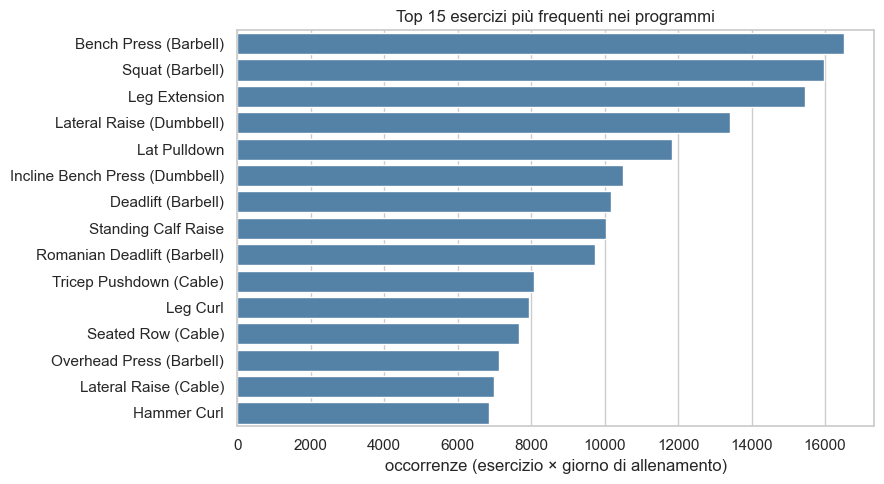
\includegraphics[width=0.78\textwidth]{images/fig_top_exercises.png}
\caption{Esercizi più frequenti nei programmi, ottenuti con tre \texttt{\$unwind}
seguiti da \texttt{\$group}/\texttt{\$sort}.}
\label{fig:top}
\end{figure}

La successione dei tre \texttt{\$unwind} ha srotolato i documenti collassati,
permettendo di tornare alle 605 mila righe di partenza; la clausola
\texttt{\$group} ha poi permesso di contarle per nome (Figura~\ref{fig:top}).
Vediamo che i primi esercizi sono esercizi multiarticolari (panca piana, squat,
stacco da terra), chiamati anche ``fondamentali'' in quanto coinvolgono molti
muscoli del corpo in un solo movimento e sono usati nella maggior parte dei
programmi di forza. Il risultato è coerente con quanto ci si poteva aspettare.

Sfruttando nuovamente la clausola \texttt{\$unwind} è possibile plottare la
distribuzione dei programmi per \texttt{level} e \texttt{goal}
(Figura~\ref{fig:levelgoal}). Notiamo che le somme superano i \num{2598} documenti
collassati, ma è normale, in quanto un piano indica più livelli e più obiettivi.
Osserviamo che il dataset non è orientato agli estremi: Beginner e Advanced hanno
molti meno piani rispetto a Novice e Intermediate. Gli obiettivi più presenti
invece risultano essere Bodybuilding (1723), Muscle \& Sculpting (936) e
Powerbuilding (905), il che conferma perché gli esercizi più presenti nei vari
piani fossero i fondamentali.

\begin{figure}[H]
\centering
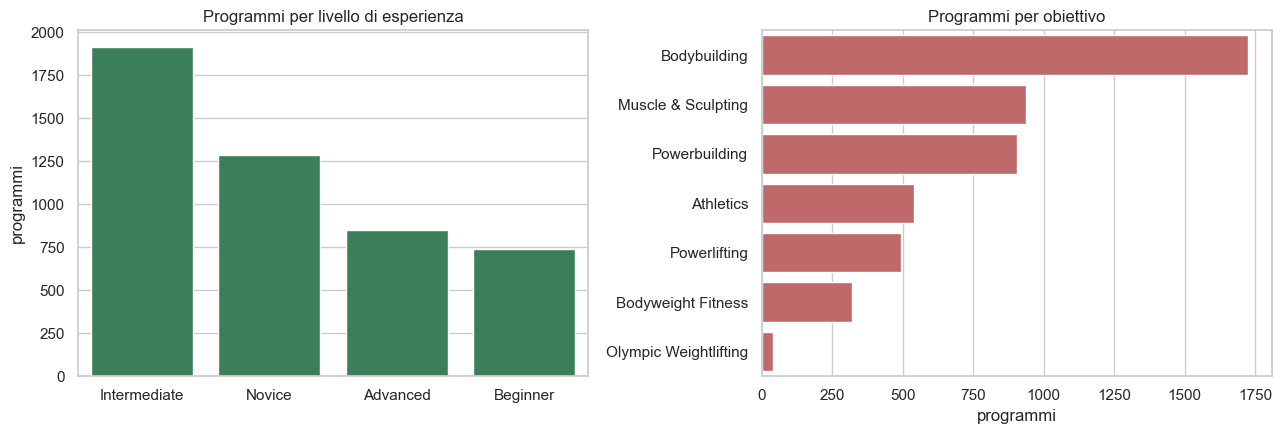
\includegraphics[width=0.92\textwidth]{images/fig_level_goal.png}
\caption{Distribuzione dei programmi per livello (sinistra) e obiettivo (destra),
ottenuta con \texttt{\$unwind} sugli array nativi \texttt{level} e \texttt{goal}.}
\label{fig:levelgoal}
\end{figure}

Con la query successiva ho stampato la distribuzione delle strutture richieste per
eseguire i programmi (Figura~\ref{fig:equip}). Questa query è stata fatta per
dimostrare che, anche usando una tecnica di embedding e quindi collassando i
documenti, possiamo usare funzioni quali \texttt{\$map} e \texttt{\$sum} al posto
di \texttt{\$unwind} per andare a lavorare \emph{dentro} gli array: è così che
calcolo le statistiche sugli esercizi per programma (media 232{,}9, min 1, max
\num{5040}). Questo dimostra il potenziale e la versatilità che vi è dietro le
aggregation expression di MongoDB. Analizzando il plot vediamo come la maggior
parte dei piani richieda una Full Gym o almeno una Garage Gym per essere eseguita.

\begin{figure}[H]
\centering
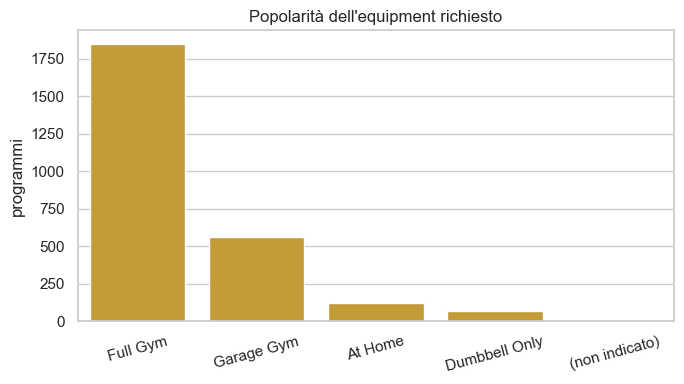
\includegraphics[width=0.7\textwidth]{images/fig_equipment.png}
\caption{Equipment richiesto dai programmi. I programmi a corpo libero o ad
attrezzatura minima sono una nicchia.}
\label{fig:equip}
\end{figure}

Infine ho voluto approfondire un aspetto molto utile di MongoDB, il
\texttt{\$facet}. Questa clausola permette di restituire un unico documento in
output basato su tutti i risultati, eseguendo più sotto-pipeline indipendenti in
una sola scansione del DB: in una passata ottengo i \num{2598} programmi totali,
la durata media (8{,}8 settimane, 69 minuti per workout), i top obiettivi e la
distribuzione per livello. Tipicamente questa tecnica viene usata in pagine di
riepilogo e/o dashboard, in quanto con una sola round-trip al database si
ottengono N metriche. Questo la rende molto simile alla funzione
\texttt{.describe()} di pandas, che in un sol colpo restituisce varie metriche del
dataframe.

\paragraph{Risposta a RQ2.} L'aggregation framework mi ha permesso di fare varie e
vaste operazioni sui dati del mio database pur mantenendo alta l'efficienza, senza
spostare i dati fuori dal database; a Python restano solo i grafici.

%==================================================================
\section{RQ3 --- Indici e performance}
\label{sec:rq3}

Quando lavoriamo con database, e soprattutto con grandi quantità di dati, è
necessario saper sfruttare gli indici messi a disposizione. Così come fatto nel
corso di Database e per Neo4j, ho deciso di implementare una sezione dedicata agli
indici anche in questo progetto.

Su MongoDB, se non vi sono indici sui campi dei documenti, quello che avviene è
una \textbf{\texttt{COLLSCAN}}: viene letta \emph{tutta} la collection e il filtro
è applicato documento per documento. Lavoro sulla collection \texttt{workouts}
piatta, non collassata, in quanto rappresenta il caso peggiore (605k documenti).
Lancio due query realistiche, la prima filtrando sul singolo campo
\texttt{exercise\_name} e la seconda applicando un doppio filtro
(\texttt{equipment}~+~\texttt{exercise\_name}), e profilo tutto usando
\textbf{\texttt{explain("executionStats")}} che, come \texttt{PROFILE} su Neo4j,
permette di vedere il piano scelto, il numero di documenti esaminati, il tempo di
esecuzione della query, ecc.

Come previsto, senza alcun indice la scansione \texttt{COLLSCAN} avviene su tutta
la collezione (\num{605033} documenti esaminati, $\sim$280~ms). Ragionando in
termini di dataset molto più grandi, come quelli utilizzati dalle grandi aziende,
query di questo tipo non sono accettabili: con l'aumentare dei dati aumenta anche
il tempo richiesto per eseguire la query. Creo dunque un indice su
\texttt{exercise\_name} e un indice composto su
\texttt{equipment}~+~\texttt{exercise\_name} e ripeto le stesse query profilandole.

\begin{table}[H]
\centering
\caption{Effetto degli indici, misurato con \texttt{explain("executionStats")} su
\texttt{workouts}.}
\label{tab:index}
\begin{tabular}{llrrr}
\toprule
Query & Piano & \texttt{docsExamined} & \texttt{nReturned} & Tempo \\
\midrule
1 campo, no indice        & \texttt{COLLSCAN}        & \num{605033} & \num{16508} & $\sim$280 ms \\
1 campo, indice singolo   & \texttt{IXSCAN}+\texttt{FETCH} & \num{16508} & \num{16508} & $\sim$40 ms \\
2 campi, indice composto  & \texttt{IXSCAN}+\texttt{FETCH} & \num{4116}  & \num{4116}  & $\sim$6 ms \\
covered query             & \texttt{IXSCAN} (no \texttt{FETCH}) & \textbf{0} & \num{4116} & $\sim$2 ms \\
\bottomrule
\end{tabular}
\end{table}

La Tabella~\ref{tab:index} riassume i risultati:
\begin{enumerate}
    \item \textbf{\texttt{IXSCAN}~+~\texttt{FETCH}:} con l'indice MongoDB naviga il
    B-tree fino alle chiavi che soddisfano il filtro
    (\texttt{keysExamined}~=~\texttt{nReturned}) e va a prendere solo quei
    documenti: \texttt{docsExamined} crolla da \num{605033} a \num{16508} e il
    tempo da $\sim$280 a $\sim$40~ms.
    \item \textbf{Indice composto:} la query sui due campi utilizza l'indice
    composto e riporta i \num{4116} documenti in $\sim$6~ms. L'ordine dei campi
    conta (\emph{prefix rule}): lo stesso indice servirebbe anche query sul solo
    \texttt{equipment}, ma non sul solo \texttt{exercise\_name}.
    \item \textbf{Covered query:} caso particolare di query in cui vengono
    richiesti solo i campi che sono nell'indice. La pipeline eseguita da MongoDB
    passa da ``lettura indice, fetch dei documenti, ritorno dei risultati'' a
    ``lettura indice e ritorno dei risultati'': \texttt{docsExamined}~$=0$, lo
    stage \texttt{FETCH} sparisce e il tempo viene ulteriormente abbattuto, in
    quanto si salta la fase più dispendiosa nell'esecuzione di una query, ovvero
    leggere effettivamente i documenti.
\end{enumerate}

Nonostante la diminuzione significativa del tempo richiesto per recuperare i dati,
creare indici comporta aggiungere strutture dati che vanno memorizzate (e che
quindi occupano spazio) e che devono essere aggiornate a ogni scrittura. Su
collezioni nelle quali vengono eseguite frequenti scritture potrebbe essere
necessario calcolarne i benefici, per capire l'effettivo guadagno.

\paragraph{Risposta a RQ3.} L'impatto è di 2--3 ordini di grandezza sui documenti
esaminati; \texttt{explain} rende la decisione misurabile invece che intuitiva.

%==================================================================
\section{RQ4 --- Il teorema CAP, sperimentato sul replica set}
\label{sec:rq4}

Il teorema CAP~\cite{GilbertLynch2002,Brewer2012CAP} dice che un sistema
distribuito, di fronte a una \textbf{partizione di rete (P)}, deve scegliere tra
essere \textbf{consistente (C)} e \textbf{disponibile (A)}. MongoDB sceglie la
consistenza: è un sistema \textbf{CP}. In questa sezione non mi limito a
dichiararlo, ma dimostro la reazione del sistema di fronte a ``guasti'' sui nodi.

Su MongoDB possiamo impostare il \textbf{write concern}, ovvero la policy secondo
la quale viene descritta la durabilità di una scrittura, ai seguenti livelli:
\begin{itemize}
    \item \texttt{w:1} (scrittura ok dopo il nodo primary);
    \item \texttt{w:2} (scrittura ok dopo primary + 1 secondary);
    \item \texttt{w:"majority"} (scrittura ok dopo che ha scritto sulla
    maggioranza dei nodi).
\end{itemize}
È possibile anche impostare la \textbf{read preference}, ovvero scegliere da quali
nodi leggere, ai seguenti valori:
\begin{itemize}
    \item \texttt{primary} (leggiamo dal nodo primario, il default);
    \item \texttt{secondary} (leggiamo dai nodi secondari);
    \item \texttt{nearest} (leggiamo dal nodo più vicino nella rete distribuita);
    \item \texttt{primaryPreferred} (preferiamo il primario, ma se è down leggiamo
    da un secondary).
\end{itemize}
Per simulare la partizione fermerò il container Docker del primary e osserveremo
cosa succede.

\paragraph{6.1 --- Write concern: quanto costa la durabilità.} Misuro il costo
della garanzia inserendo gli stessi batch (500 documenti $\times$ 5 run) con i due
livelli estremi: \texttt{w:"majority"} paga un ``sovrapprezzo'' rispetto a
\texttt{w:1} (20{,}1 contro 15{,}6~ms medi per batch), perché la conferma deve
attendere la replica su almeno un secondary. Su localhost il divario è di pochi
millisecondi, ma in un cluster geo-distribuito diventa la latenza di rete tra
datacenter. In cambio \texttt{majority} garantisce che la scrittura
\textbf{sopravviva a un failover}, in quanto una scrittura confermata solo con
\texttt{w:1} viene annullata (rollback) se il primary cade prima di replicarla.
Questo rappresenta proprio il trade-off tra C e A: più aggiungiamo garanzie di
consistenza, più aumenta la latenza.

\paragraph{6.2 --- Read preference: leggere dai secondary.} Con
\texttt{readPreference=secondary} il driver instrada la lettura su un nodo
secondario: nell'esperimento la stessa query viene servita dalla porta 27017
(primary) o 27018 (secondary) a seconda della preference, e il count sui due nodi
coincide (\num{605033} documenti, la replica è al passo). Il prezzo è la
\textbf{consistenza eventuale}: i secondary applicano l'oplog in modo asincrono,
quindi una lettura può restituire dati \emph{stale} di qualche istante.

\paragraph{6.3 --- Failover: il cluster perde il primary.} L'esperimento centrale
della RQ4. Uccido il container del primary con \textbf{\texttt{docker kill}} e,
una volta al secondo, provo a \textbf{scrivere} (timeout 2~s) e a \textbf{leggere
da un secondary}, registrando gli esiti su una timeline.

Perché \texttt{kill} e non \texttt{stop}? Con \texttt{docker stop} il
\texttt{mongod} riceve un SIGTERM e fa uno stepdown graceful: avvisa i secondary,
che eleggono il nuovo primary quasi istantaneamente (l'ho verificato, e la
finestra di indisponibilità è praticamente invisibile). È il meccanismo usato nei
riavvii pianificati. Il teorema CAP però parla di guasti \emph{non pianificati}:
usando \texttt{docker kill} mi assicuro che il segnale sia un SIGKILL, e questo fa
partire il timeout di default di 10~s (\texttt{electionTimeoutMillis}) prima che i
secondary, accortisi della scomparsa del primary tramite gli heartbeat falliti,
indicano l'elezione~\cite{Ongaro2014Raft}.

La timeline mostra il comportamento CP di MongoDB in diretta: nella mia run i
primi tre tentativi di scrittura (a $t=0$, 3 e 6~s) falliscono, e a $t\approx9$~s
la scrittura torna OK sul nuovo primary (il nodo sulla porta 27018).
\begin{itemize}
    \item \textbf{Le scritture si bloccano} per l'intera durata dell'elezione
    ($\sim$10~s): il driver non trova un primary
    (\texttt{ServerSelection\allowbreak Timeout\allowbreak Error}) perché al
    momento non esiste. Il sistema sacrifica la disponibilità in scrittura pur di
    non rischiare due primary concorrenti (\emph{split-brain}).
    \item \textbf{Le letture dai secondary continuano} per tutto il tempo: la
    disponibilità in lettura non cambia.
    \item I due nodi superstiti formano ancora la \textbf{maggioranza} (2 su 3),
    quindi possono eleggere un nuovo primary e il servizio riprende da solo. Se
    avessi fermato \emph{due} nodi, il nodo superstite sarebbe rimasto secondary
    per sempre: nessuna maggioranza, nessun primary, niente scritture.
\end{itemize}

Il vecchio primary, riavviato, \textbf{rientra nel replica set come SECONDARY}: si
risincronizza dal nuovo primary e recupera le scritture perse durante la sua
assenza. Nessun intervento manuale.

\begin{table}[H]
\centering
\caption{Mappatura degli eventi osservati sul teorema CAP.}
\label{tab:cap}
\begin{tabular}{p{7.2cm}p{8.0cm}}
\toprule
Evento osservato & Lettura CAP \\
\midrule
Scritture bloccate durante l'elezione ($\sim$10~s) & sotto partizione MongoDB
sacrifica \textbf{A} per \textbf{C} $\rightarrow$ sistema \textbf{CP} \\
\texttt{w:"majority"} più lento di \texttt{w:1} & il \emph{grado} di C si paga in
latenza, scrittura per scrittura \\
Serve la maggioranza per eleggere il primary & protezione dallo split-brain: mai due
``verità'' divergenti \\
\bottomrule
\end{tabular}
\end{table}

\paragraph{Risposta a RQ4.} La mappa completa è in Tabella~\ref{tab:cap}: CAP per
MongoDB non è un'etichetta statica, ma una manopola. Write concern e read
preference permettono di scegliere, per singola operazione, quanto pagare in
latenza e disponibilità per la consistenza.

%==================================================================
\section{Conclusioni}
\label{sec:conclusioni}

In questo approfondimento ho esplorato MongoDB sui quattro assi delle research
question, con esperimenti riproducibili su un replica set Docker a 3 nodi:
\begin{itemize}
    \item \textbf{RQ1 --- Modellazione.} Il dataset piatto (605k righe con
    metadati duplicati) è stato rimodellato in \num{2598} documenti annidati
    programma $\rightarrow$ settimane $\rightarrow$ giorni $\rightarrow$ esercizi
    \emph{con una sola pipeline di aggregazione} (\texttt{\$group}~$\times$3 +
    \texttt{\$out}). Risultato: dati logici da 414 a 54~MB ($-87\%$) e l'intero
    programma recuperabile con una singola lettura atomica ($\sim$1{,}2~ms contro
    $\sim$165). L'embedding vince quando l'unità di accesso coincide con il
    documento; il referencing resta preferibile per sotto-oggetti condivisi o
    array a crescita illimitata (limite BSON 16~MB).
    \item \textbf{RQ2 --- Aggregation framework.} Tutta l'analisi descrittiva
    (top esercizi, distribuzioni per livello/obiettivo/equipment, statistiche
    multi-metrica con \texttt{\$facet}) è stata eseguita dentro il database:
    \texttt{\$unwind} riapre la gerarchia quando serve la granularità fine,
    \texttt{\$map}/\texttt{\$size} navigano gli array senza esploderli.
    \item \textbf{RQ3 --- Indici.} Con \texttt{explain("executionStats")} ho
    misurato il passaggio da \texttt{COLLSCAN} (605k documenti esaminati) a
    \texttt{IXSCAN} (solo i documenti restituiti) fino alla covered query
    (\texttt{docsExamined}~$=0$): 2--3 ordini di grandezza, al costo di spazio e
    overhead in scrittura.
    \item \textbf{RQ4 --- CAP.} Il failover dal vivo ha mostrato il carattere
    \textbf{CP} di MongoDB: alla caduta del primary le scritture si bloccano per i
    $\sim$10 secondi dell'elezione (consistenza pagata in disponibilità), le
    letture dai secondary proseguono in consistenza eventuale, e write concern e
    read preference permettono di regolare il trade-off per singola operazione.
\end{itemize}

Il filo conduttore è che le scelte di design di MongoDB (documenti, pipeline,
indici, replica) diventano comprensibili solo guardando \emph{cosa ottimizzano}:
il modello documentale ottimizza il pattern di accesso, l'aggregation evita di
muovere i dati, gli indici comprano letture con scritture, il replica set compra
consistenza con disponibilità. Strumenti come \texttt{explain},
\texttt{collStats} e \texttt{replSetGetStatus} rendono ognuno di questi trade-off
misurabile, ed è questo che li rende decisioni ingegneristiche e non atti di fede.
La sperimentazione completa, con istruzioni di installazione e uso, è pubblicata
sul repository indicato in nota al titolo.

%==================================================================
\newpage
\addcontentsline{toc}{section}{Riferimenti bibliografici}
\bibliographystyle{apalike}
\bibliography{ref}

%==================================================================
\newpage
\appendix
\section{Dettagli di riproduzione}
\label{app:repro}

Il repository contiene il notebook \texttt{fitness\_exercise\_analysis.ipynb}, il
\texttt{docker-compose.yml} del replica set, lo script \texttt{rs-init.js} di
inizializzazione e un README con i passi dettagliati. In sintesi:

\begin{lstlisting}[language=bash, caption={Avvio del replica set e inizializzazione.}]
# 1. avvio dei tre nodi
docker compose up -d
# 2. inizializzazione del replica set (solo la prima volta)
docker compose exec mongo1 mongosh --port 27017 --quiet /rs-init.js
# 3. verifica: 3 membri, 1 PRIMARY
docker compose exec mongo1 mongosh --port 27017 --quiet \
  --eval 'rs.status().members.forEach(m => print(m.name, m.stateStr))'
\end{lstlisting}

\begin{lstlisting}[language=bash, caption={Ambiente Python e dati.}]
python3 -m venv venv && source venv/bin/activate
pip install -r requirements.txt
cp .env.example .env          # connection string del replica set
# il dataset (294 MB) va scaricato da Kaggle in archive/
jupyter lab                   # eseguire le celle in ordine
\end{lstlisting}

Il dataset non è incluso nel repository (294~MB, cartella \texttt{archive/} in
\texttt{.gitignore}): va scaricato da Kaggle~\cite{BoostcampDataset} e collocato in
\texttt{archive/programs\_detailed\_boostcamp\_kaggle.csv}. Il notebook esegue
dall'alto senza errori contro il replica set; la cella di RQ4 richiede Docker
attivo sulla macchina che ospita il notebook, perché ferma e riavvia un container
via \texttt{subprocess}.

\end{document}
